\documentclass[11pt, a4paper]{article}
\usepackage[a4paper, margin=2.5cm]{geometry}
\usepackage[english]{babel}
\usepackage{amsmath, mathtools, amssymb, booktabs, amsthm}
\usepackage{enumitem}
\usepackage{mathrsfs}
\usepackage{dsfont}
\usepackage{cancel}
\usepackage{xcolor}
\usepackage{etoolbox}
\usepackage{needspace}
\usepackage{framed}
\usepackage{tikz}
\usetikzlibrary{patterns}
\usepackage[framemethod=TikZ]{mdframed}

% Raccourcis
\newcommand{\ind}{\mathds{1}}
\newcommand{\KL}{\mathrm{KL}}
\newcommand{\annot}[1]{\textcolor{gray}{\text{#1}}}
% accolade grise (pour les annotations grises)
\newcommand{\gunderbrace}[2]{{\color{gray}\underbrace{\color{black}#1}_{#2}}}
\newcommand{\circled}[1]{\tikz[baseline=(c.base)]\node[draw,circle,inner sep=0.6pt,font=\scriptsize](c){#1};}
% Parties à rédiger à la main
% Contrainte nommée (C_k) accumulée dans une preuve
\newcommand{\constraint}[2]{\[ (\mathrm{C}_{#1}) \qquad #2 \]}
\newcommand{\tocomplete}[1][]{\noindent\textcolor{red}{\textbf{TO COMPLETE\ifx&#1&\else: #1\fi}}}


% Configuration des listes
\setlist[itemize]{label=-}

% Compteur commun (numérotation par section, comme avant)
\newcounter{theorem}[section]
\renewcommand{\thetheorem}{\thesection.\arabic{theorem}}

% Environnements encadrés (mdframed) avec onglet de titre
% #1 : nom de l'environnement, #2 : intitulé, #3 : couleur
\newcommand{\newmdtheorem}[3]{%
\newenvironment{#1}[1][]{%
\refstepcounter{theorem}%
\ifstrempty{##1}%
{\mdfsetup{%
frametitle={%
\tikz[baseline=(current bounding box.east),outer sep=0pt]
\node[anchor=east,rectangle,fill=#3]
{\strut #2~\thetheorem};}}
}%
{\mdfsetup{%
frametitle={%
\tikz[baseline=(current bounding box.east),outer sep=0pt]
\node[anchor=east,rectangle,fill=#3]
{\strut #2~\thetheorem:~##1};}}%
}%
\mdfsetup{innertopmargin=10pt,linecolor=#3,%
linewidth=2pt,topline=true,%
frametitleaboveskip=\dimexpr-\ht\strutbox\relax
}
\needspace{5\baselineskip}%
\begin{mdframed}[]\relax\setlength{\parindent}{0pt}%
}{\end{mdframed}}%
}

\newmdtheorem{theorem}{Theorem}{red!25}
\newmdtheorem{lemma}{Lemma}{yellow!50}
\newmdtheorem{proposition}{Proposition}{orange!30}
\newmdtheorem{corollary}{Corollary}{orange!60}

% Preuve et barres verticales
% Les barres sont faites avec leftbar du package framed (\MakeFramed). framed
% ne sait pas couper un cadre imbriqué dans un autre : chaque \begin/\end{leftbar}
% ferme donc le morceau encadré courant et en rouvre un au premier niveau, dessiné
% avec autant de barres que de niveaux ouverts (et le cadre de la preuve autour).
% Tous les morceaux peuvent ainsi se couper entre les pages. La preuve est
% construite de la même façon (et non avec mdframed) pour la même raison.
\makeatletter
\newcount\lb@depth
\newif\iflb@inproof
\newif\iflb@top
\newif\iflb@bottom
\newcommand{\prooftitle}{}
% Un morceau : #1 = avec titre et ligne du haut, #2 = avec ligne du bas, #3 = contenu
\newcommand{\lb@piece}[3]{%
\iflb@inproof\def\lb@pad{10pt}\else\def\lb@pad{0pt}\fi
\ifnum#1=1 \def\lb@up{18pt}\else\def\lb@up{2pt}\fi
\ifnum#2=1 \def\lb@down{-6pt}\else\def\lb@down{-2pt}\fi
\begin{tikzpicture}
\node[inner xsep=\lb@pad, inner ysep=0pt, outer sep=0pt] (c)
  {\hbox{\hskip\dimexpr9pt*\lb@depth\relax#3}};
\coordinate (t) at ([yshift=\lb@up]c.north west);
\coordinate (u) at ([yshift=\lb@up]c.north east);
\coordinate (b) at ([yshift=\lb@down]c.south west);
\coordinate (e) at ([yshift=\lb@down]c.south east);
\ifnum\lb@depth>\z@
  \foreach \k in {1,...,\lb@depth}
    \draw[gray!70, line width=1pt]
      ([xshift=\lb@pad+(\k-1)*9pt+0.5pt]t) -- ([xshift=\lb@pad+(\k-1)*9pt+0.5pt]b);
\fi
\iflb@inproof
  \ifnum#2=1
    \draw[gray!20, line width=2pt] (t) -- (b) -- (e) -- (u);
  \else
    \draw[gray!20, line width=2pt] (t) -- (b) (e) -- (u);
  \fi
  \ifnum#1=1
    \draw[gray!20, line width=2pt] (t) -- (u);
    \node[anchor=west, fill=gray!20] at ([xshift=10pt]t) {\strut\itshape\prooftitle};
  \fi
\fi
\end{tikzpicture}}
\newif\iflb@open
\newcommand{\lb@open}{%
\global\lb@opentrue
% dans une preuve, seul le premier morceau peut commencer une nouvelle page
% (framed coupe lui-même un morceau trop long)
\iflb@inproof\iflb@top\else\@nobreaktrue\fi\fi
\def\FrameCommand{\lb@piece{\iflb@top1\else0\fi}{\iflb@bottom1\else0\fi}}%
\def\FirstFrameCommand{\lb@piece{\iflb@top1\else0\fi}{0}}%
\def\MidFrameCommand{\lb@piece{0}{0}}%
\def\LastFrameCommand{\lb@piece{0}{\iflb@bottom1\else0\fi}}%
\MakeFramed{\advance\hsize-\width\FrameRestore\setlength{\parindent}{0pt}}}
% Un morceau resté vide (par ex. entre deux \end{leftbar}) est abandonné
\newcommand{\lb@discard}{\global\lb@openfalse\egroup}
\newcommand{\lb@dropempty}{%
\iflb@open\ifvmode\ifnum\lastnodetype=\m@ne\iflb@top\else\lb@discard\fi\fi\fi\fi}
\newcommand{\lb@close}{%
\lb@dropempty
\iflb@open\global\lb@openfalse\endMakeFramed\global\lb@topfalse\global\@nobreakfalse\fi}
\newcommand{\lb@reopen}{%
\iflb@inproof\lb@open\else\ifnum\lb@depth>\z@\lb@open\fi\fi}
% Bas du cadre de la preuve quand elle se termine juste après une leftbar
% (dessiné en surimpression si la page est pleine, pour ne pas partir seul
% sur la page suivante)
\newcommand{\lb@finalpiece}{%
\dimen@\pagegoal\advance\dimen@-\pagetotal
\nointerlineskip
\centerline{\begin{tikzpicture}[\ifdim\dimen@<14pt overlay\fi]
\useasboundingbox (0,-12pt) rectangle (\textwidth,0pt);
\draw[gray!20, line width=2pt] (1pt,0pt) -- (1pt,-11pt) -- (\textwidth-1pt,-11pt) -- (\textwidth-1pt,0pt);
\node[anchor=east] at (\textwidth-11pt,-5pt) {\qedsymbol};
\end{tikzpicture}}}
\renewcommand{\leftbar}{%
\endgroup
\lb@close
\begingroup\def\@currenvir{leftbar}%
\OuterFrameSep=\z@\edef\FrameHeightAdjust{\the\baselineskip}%
\global\advance\lb@depth\@ne
\lb@open}
\renewcommand{\endleftbar}{%
\lb@close
\global\advance\lb@depth\m@ne
\aftergroup\lb@reopen}

\renewenvironment{proof}[1][\proofname]{%
\par\needspace{5\baselineskip}\addvspace{\topsep}%
\def\prooftitle{#1}\pushQED{\qed}%
\OuterFrameSep=\z@\edef\FrameHeightAdjust{\the\baselineskip}%
% sinon \vsplit laisse dépasser la profondeur d'une grande équation en bas de page
\splitmaxdepth=\z@
% pas de saut de page entre deux morceaux
\def\fb@afterframe{\nointerlineskip\null\penalty\@M\vskip\OuterFrameSep\relax}%
\global\lb@inprooftrue\global\lb@toptrue\global\lb@bottomfalse
\lb@open}%
{\lb@dropempty
\iflb@open\popQED\global\lb@bottomtrue\lb@close\else\lb@finalpiece\fi
\global\lb@inprooffalse
\par\penalty\z@\addvspace{\topsep}}
\makeatother

\newmdtheorem{definition}{Definition}{cyan!25}
\newmdtheorem{example}{Example}{gray!35}

% Environnement non numéroté : #1 nom, #2 titre par défaut, #3 couleur
\newcommand{\newmdbox}[3]{%
\newenvironment{#1}[1][#2]{%
\mdfsetup{%
frametitle={%
\tikz[baseline=(current bounding box.east),outer sep=0pt]
\node[anchor=east,rectangle,fill=#3]
{\strut ##1};},
innertopmargin=10pt,linecolor=#3,%
linewidth=2pt,topline=true,%
frametitleaboveskip=\dimexpr-\ht\strutbox\relax
}%
\needspace{5\baselineskip}%
\begin{mdframed}[]\relax\setlength{\parindent}{0pt}%
}{\end{mdframed}}%
}

\newmdbox{intuition}{Intuition}{green!30}

\begin{document}

\part{Bayesian Modelling and Decision Theory}

\section{Bayesian Formulation}

\subsection{Frequentist Approach}
Loss function $l(\theta, \delta)$, frequentist risk function:
\[ R(\theta,\delta) = \text{function of } \theta = E[l(\theta,\delta(X))] = \int_{\mathcal{X}} l(\theta,\delta(x)) dP_X \]

\subsection{Bayesian Statistics}
$\theta$ unknown modelled as a r.v.

$(\Theta, \mathcal{A}, \pi)$ probability space for $\theta$, where:
\begin{itemize}
    \item $\mathcal{A}$: $\sigma$-field
    \item $\pi$: prior probability
    \item $X|\theta \sim P_{\theta}$ conditional distribution of $X$ given $\theta$.
\end{itemize}
Prior $\pi \implies (X, \theta) \sim P_{\Theta} \times \pi$

\begin{example}
Let $\pi(\theta|x)$ be the conditional distribution of $\theta$ given $X$, i.e., the posterior distribution.

Non-parametric bayesian stat:
\[ f(x) = \sum_{j \in \mathbb{N}} c_j \varphi_j(x), \quad (c_j)_{j \in \mathbb{N}} \]
For example:
$J \sim \text{Poisson}(\lambda)$; $\forall i \in (0,2)$
\[ f(x, \theta) = \sum_{j=1}^{n} \pi_J(j) d\pi(f_{\theta,j}|J=j) \]
\end{example}

\begin{definition}[Dominated Model]
Model $\mathcal{P} = \{P_\theta, \theta \in \Theta\}$ for observations $X \in \mathcal{X}$ is a dominated model if $\exists \mu$ measure on $\mathcal{X}$ such that $\forall \theta \in \Theta$:
\[ P_\theta \ll \mu \quad \text{(absolutely continuous)} \]
$f_\theta = \frac{dP_\theta}{d\mu}$ (density). Same $\mu$ for all $\theta$ ($\mu \neq 0$ in general).
\end{definition}

\begin{theorem}[Bayes Theorem]
If $P_\theta \ll \mu \quad \forall \theta \in \Theta$, and if $\pi$ is a probability measure with density w.r.t. $\nu$ on $\Theta$, then the posterior has a density w.r.t. $\nu$:
\[ \pi(\theta|x) = \frac{f_\theta(x)\pi(\theta)}{\int_{\Theta} f_\theta(x)\pi(\theta)d\nu(\theta)} \]
\end{theorem}

\begin{example}[Poisson Distribution] 
$X_1, \dots, X_n \sim \mathcal{P}(\theta)$ (Poisson $\theta$), where $X_i \in \mathbb{N}$:
\[ P_\theta(X=k) = e^{-\theta} \frac{\theta^k}{k!} \]
Prior $\pi_b(\theta) = b e^{-b\theta}, \quad \theta > 0$ (density w.r.t. Lebesgue on $\mathbb{R}$). 

$\pi_b = \mathcal{E}(b)$

Posterior has a density w.r.t. Lebesgue:
\[ \pi(\theta | x_1, \dots, x_n) = \frac{\prod_{i=1}^{n} P_\theta(X_i=x_i) b e^{-b\theta}}{\int_{0}^{\infty} \prod_{i=1}^{n} P_{\tilde{\theta}}(X_i=x_i) b e^{-b\tilde{\theta}} d\tilde{\theta}} \]
\[ \pi(\theta | x_1, \dots, x_n) \propto e^{-(n+b)\theta} \theta^{\sum x_i} \]
\[ \equiv \Gamma\left(\sum_{i=1}^{n}x_i + 1, n+b\right) \]
Recall $\Gamma(a', b')$ has a density w.r.t. Lebesgue:
\[ \pi_{a',b'}(y) = e^{-b'y} y^{a'-1} \frac{(b')^{a'}}{\Gamma(a')} \mathbb{I}_{y>0} \]
\end{example}

\begin{example}[Normal Distribution]
$X_1, \dots, X_n$ i.i.d. $\mathcal{N}(\theta, 1)$, $\theta \in \mathbb{R}$

$\mu = \text{Lebesgue on } \mathbb{R}^n$

$\nu = \text{Lebesgue on } \mathbb{R}$

Prior $\theta \sim \mathcal{N}(\mu_0, \tau_0^2)$

Posterior density $\pi(\theta | X)$:
\[ \propto \prod_{i=1}^{n} \exp\left(-\frac{(X_i-\theta)^2}{2}\right) \times \exp\left(-\frac{(\theta-\mu_0)^2}{2\tau_0^2}\right) \]
\[ \propto \exp\left(-\frac{\theta^2}{2}\left(n+\frac{1}{\tau_0^2}\right) + \theta\left(n\overline{X}_n + \frac{\mu_0}{\tau_0^2}\right)\right) \]
\[ \equiv \mathcal{N}\left(\frac{n\overline{X}_n + \frac{\mu_0}{\tau_0^2}}{n + \frac{1}{\tau_0^2}}, \frac{1}{n + \frac{1}{\tau_0^2}}\right) \]
\end{example}

\begin{definition}[Conjugate Family]
If the prior $\pi$ belongs to $\mathcal{S}$, a family of distributions such that the posterior $\pi(\cdot|x) \in \mathcal{S}$ a.s., then $\mathcal{S}$ is called a conjugate family of priors w.r.t. the statistical model we are using.
\end{definition}

\begin{example}
$X_1, \dots, X_n \sim \mathcal{P}(\theta)$, $\theta > 0$

$\mathcal{S} := \left\{ \pi_{a,b}(\theta) = \frac{\theta^{a-1}e^{-b\theta}b^a}{\Gamma(a)} \right\} \equiv \Gamma \text{ distrib}$

Then $\forall n$: $\pi(\theta | x_1, \dots, x_n) \sim \Gamma\left(a + n\overline{x}_n, b + n\right) \in \mathcal{S}.$
\end{example}

If the model is dominated, posterior density w.r.t. $\nu$:
\[ \pi(\theta|x) = \frac{f_\theta(x)\pi(\theta)}{m_\pi(x)} \propto f_\theta(x)\pi(\theta) \]
$m_\pi(x)$ is the marginal density of the data (marginal likelihood).

\subsection{Hierarchical Prior}
$\pi = \pi_\lambda$ (e.g. $\Gamma(a, b)$ with $\lambda = (a,b)$).

$\lambda$ is called a hyperparameter.

\begin{example}
$X_i \sim \mathcal{N}(\theta_i, 1)$ for $i=1, \dots, n$

$\theta = (\theta_1, \dots, \theta_n)$

$\theta_i \sim \mathcal{N}(0, \tau^2)$

$X_i \in \mathbb{R}$

$\tau^2$ is here a hyperparameter that has a lot of influence. 
\begin{itemize}
    \item Choice 1: fix $\tau^2$ arbitrarily.
    \item Choice 2: take $\tau^2 \sim \text{Cauchy}$ (positive part). Fat tails, so that $\tau^2$ is sufficiently large.
\end{itemize}
\end{example}

\section{Bayesian Decision Theory}

\subsection{Loss and Risks}
Model $\mathcal{P}_\theta, \theta \in \Theta$ for observations $X$.

\begin{definition}[Loss Function]
A loss function $l: \Theta \times \mathcal{D} \rightarrow \mathbb{R}_+$, where $\mathcal{D}$ represents decisions $\delta$.
\end{definition}

\begin{example}[Loss Functions]
\begin{enumerate}
    \item If $\mathcal{D} = \Theta$:
    \begin{itemize}
        \item Quadratic loss: $l(\theta,\delta) = \|\theta - \delta\|^2$
        \item $L_1$ loss: $l(\theta,\delta) = \|\theta - \delta\|_1 = \sum_{j=1}^{d} |\theta_j - \delta_j|, \quad \theta \in \mathbb{R}^d$
    \end{itemize}
    \item If $\mathcal{D} = \{g(\theta), \theta \in \Theta\}$, $g: \Theta \rightarrow \mathbb{R}$:
    \begin{itemize}
        \item $l(\theta,\delta) = \|g(\theta) - \delta\|^2$
        \item $l(\theta,\delta) = \|g(\theta) - \delta\|_1$
    \end{itemize}
    \item Test $\mathcal{D} = \{0, 1\}$:
    \begin{itemize}
        \item ex: $H_0: \theta \in \Theta_0$ vs $H_1: \theta \in \Theta_1$
        \item $\Theta_0 \cap \Theta_1 = \emptyset$
        \item $l(\theta,\delta) = 1 \text{ if } \theta \text{ and } \delta \text{ disagree, } 0 \text{ otherwise.}$
    \end{itemize}
    \item $X_1, \dots, X_n \sim f_\theta$ density w.r.t. Lebesgue:
    \begin{itemize}
        \item $l(\theta, \delta) = \text{KL}(f_\theta, f_\delta)$ (with $\delta = \Theta$)
    \end{itemize}
\end{enumerate}
\end{example}

\begin{definition}[Risks]
\begin{itemize}
    \item \textbf{Posterior risk} associated with decision $\delta$:
    \[ \rho(\pi, \delta|x) = \int_{\Theta} l(\theta, \delta) \pi(d\theta|x) \]
    \item \textbf{Integrated risk}:
    \[ r(\pi, \delta) = \int \rho(\pi, \delta|x) m_\pi(dx) \]
    (where $m_\pi$ is the marginal distribution of $X$).
\end{itemize}
\end{definition}

\begin{definition}[Bayesian Estimator]
\[ \delta^\pi(x) := \text{argmin}_\delta \rho(\pi, \delta|x) \quad \text{for all } x \]
\end{definition}

\begin{lemma}
For any estimator $\delta$, $r(\pi, \delta^\pi) \le r(\pi, \delta)$
\end{lemma}
\begin{proof}
For all $x$, $\rho(\pi, \delta^\pi|x) \le \rho(\pi, \delta(x)|x)$
\[ \implies \int \rho(\pi, \delta^\pi|x) m_\pi(dx) \le \int \rho(\pi, \delta(x)|x) m_\pi(dx) \]
\end{proof}

\begin{lemma}
If the model is dominated by $\mu$,
\[ r(\pi, \delta) = \int_{\Theta} R(\theta, \delta) \pi(d\theta) \]
\end{lemma}
\begin{proof}[Proof (Fubini Theorem)]
\begin{align*}
r(\pi, \delta) &= \int_{\mathcal{X}} \int_{\Theta} l(\theta, \delta(x)) \frac{f_\theta(x)}{m_\pi(x)} \pi(d\theta) m_\pi(x) d\mu(x) \\
&= \int_{\Theta} \left( \int_{\mathcal{X}} l(\theta, \delta(x)) f_\theta(x) d\mu(x) \right) \pi(d\theta) \\
R(\theta, \delta) &= E[l(\theta, \delta(X))]
\end{align*}
\end{proof}

\begin{example}[Quadratic Loss]
Quadratic loss, $X|\theta \sim P_\theta$, $\theta \in \Theta \subset \mathbb{R}^d$

$l(\theta, \delta) = \|\theta - \delta\|^2$

Prior $\theta \sim \pi$

Posterior: $\pi(d\theta|x) = \frac{f_\theta(x)d\pi(\theta)}{\int_\Theta f_\theta(x)d\pi(\theta)}$

$\delta \rightarrow \rho(\pi, \delta|x)$ is convex.
\[ \frac{\partial}{\partial \delta} \rho(\pi, \delta|x) = -2 \int_{\Theta} (\theta - \delta) \pi(d\theta|x) = 0 \]
\[ \implies \delta(x) = \delta^\pi(x) = \int_{\Theta} \theta d\pi(\theta|x) \]
which is the posterior mean.
\end{example}

\begin{example}[0-1 Loss]
$\Theta = \{1, \dots, K\}$

$f_\theta$ density

Prior: $\pi = (\pi_1, \dots, \pi_K)$

Loss: $l(\theta, \delta) = 1 \text{ if } \theta \neq \delta$, and $=0 \text{ if } \theta = \delta$.

\[ \rho(\pi, \delta|x) = \sum_{k=1}^{K} l(k, \delta) \pi(k|x) \]
\[ = \sum_{k=1}^{K} \mathbb{I}_{k \neq \delta} \pi(k|x) = 1 - \pi(\delta|x) \]
\[ \delta^\pi(x) = \text{argmin}_\delta (1 - \pi(\delta|x)) = \text{argmax}_k \pi(k|x) \]
\end{example}

\subsection{Admissibility}

\begin{definition}[Admissibility]
\tocomplete
\end{definition}

\begin{example}[The MLE is not admissible for $d = 3$]
\tocomplete
\end{example}
\begin{proof}
\tocomplete
\end{proof}

\subsection{Intrinsic Losses}
\tocomplete

\begin{example}[Kullback--Leibler Divergence]
\tocomplete
\end{example}
\begin{proof}[Proof (invariance of the KL divergence)]
\tocomplete
\end{proof}

\subsection{The MAP Estimator in Dominated Models}
\tocomplete

\begin{definition}[Maximum A Posteriori (MAP) Estimator]
\tocomplete
\end{definition}

\noindent\textbf{Remark:} \tocomplete

\noindent\textbf{Exercise (MAP estimator, exponential model with Gamma prior):} \tocomplete

\subsection{Improper Priors}

\begin{definition}[Improper Prior]
\tocomplete
\end{definition}

\begin{example}[Lebesgue Measure on $\mathbb{R}$]
\tocomplete
\end{example}

\tocomplete[posterior distribution associated with an improper prior]

\begin{example}[Flat Prior on a Normal Mean]
\tocomplete
\end{example}

\noindent\textbf{Exercise (normal model with prior $\pi(\mu, \sigma^2) = 1/\sigma^2$):} \tocomplete

\begin{example}[Haldane Prior for a Bernoulli Model]
\tocomplete
\end{example}

\subsubsection{Jeffreys Prior}
\tocomplete[why use improper priors, flatness and parametrization]

\begin{definition}[Jeffreys Prior]
\tocomplete
\end{definition}

\begin{proposition}[Invariance under Reparametrization]
\tocomplete
\end{proposition}
\begin{proof}
\tocomplete
\end{proof}

\noindent\textbf{Exercise (Jeffreys prior for $\mathcal{N}(\mu, 1)$):} \tocomplete

\subsection{Nuisance Parameters: Marginal Likelihoods}

\begin{definition}[Marginal Likelihood and Profile Likelihood]
\tocomplete
\end{definition}

\begin{example}[Normal Model with Unknown Variance]
\tocomplete
\end{example}

\subsection{Bayesian Tests}
\tocomplete

\begin{example}[Test in a Linear Regression]
\tocomplete
\end{example}

\tocomplete[Bayes test under the 0-1 loss]

\begin{definition}[Bayes Factor]
\tocomplete
\end{definition}

\noindent\textbf{Remark (Bayes test and Bayes factor):} \tocomplete

\begin{example}[Two Simple Hypotheses]
\tocomplete
\end{example}

\begin{example}[Point Null Hypothesis]
\tocomplete
\end{example}

\noindent\textbf{Remark (marginal likelihoods $m_0$ and $m_1$):} \tocomplete

\begin{proposition}[Bayes Test, General Case]
\tocomplete
\end{proposition}

\noindent\textbf{Remark (improper priors and the Bayes test):} \tocomplete
\begin{proof}
\tocomplete
\end{proof}

\subsection{Model Selection}
\tocomplete

\begin{example}[Variable Selection in Linear Regression]
\tocomplete
\end{example}

\noindent\textbf{Exercise (posterior distribution on the model $\gamma$):} \tocomplete

\begin{example}[Number of Components in a Mixture]
\tocomplete
\end{example}

\subsection{Other Losses for Tests}
\tocomplete

\noindent\textbf{Exercise (Bayes estimator for this loss):} \tocomplete

\subsection{Credible Regions}

\begin{definition}[Confidence Region (Frequentist Recall)]
\tocomplete
\end{definition}

\begin{definition}[Credible Region]
\tocomplete
\end{definition}

\begin{lemma}[Credible Regions are Confidence Regions on Average]
\tocomplete
\end{lemma}
\begin{proof}
\tocomplete
\end{proof}

\begin{example}[Equal-Tail Credible Interval]
\tocomplete
\end{example}

\begin{example}[Credible Interval in the Normal Model]
\tocomplete
\end{example}

\begin{definition}[Highest Posterior Density (HPD) Region]
\tocomplete
\end{definition}

\begin{theorem}[HPD Regions Minimize the Volume]
\tocomplete
\end{theorem}
\begin{proof}
\tocomplete
\end{proof}

\begin{example}[Computation of an HPD Region]
\tocomplete
\end{example}

\part{Consistency and Convergence Rate}

\section{Consistency}

\tocomplete[reminder on consistency of an estimator in frequentist evaluation]

\subsection{Definition}

Let $X_{1:n} \sim P_\theta^{(n)}$, $\theta \in \Theta$, $(\Theta, d)$ = metric Polish space.

$\pi$ = proba prior and $\pi(\cdot \mid X^{(n)}) \equiv$ posterior distribution.

\begin{definition}[Posterior Consistency]
The posterior is a.s. \emph{consistent at $\theta_0$} (w.r.t. the metric $d$) iff
\[ \forall \varepsilon > 0, \quad \pi\big(\{\theta,\ d(\theta,\theta_0) \le \varepsilon\} \,\big|\, X^{(n)}\big) \xrightarrow[n\to\infty]{} 1 \quad P_{\theta_0}^{(\infty)} \text{ a.s.} \]
\end{definition}

\tocomplete[consistency in probability]

\begin{intuition}
$X_{1:n} \sim P_{\theta_0}^{(n)}$
\begin{center}
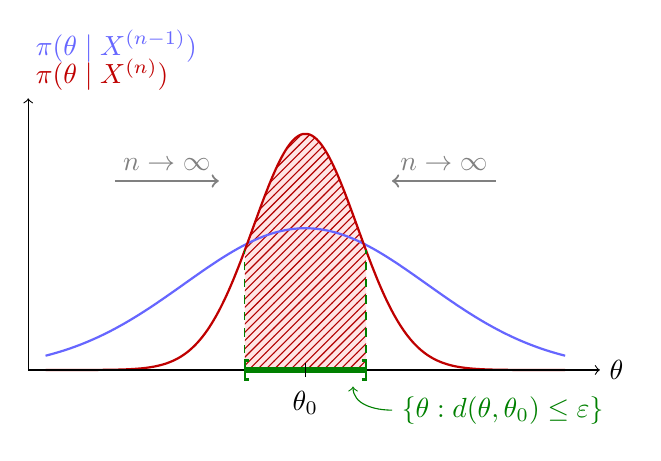
\begin{tikzpicture}[x=1.1cm, y=3cm,
  dens/.style={domain=0.2:6.2, samples=120, smooth}]
  % aire hachurée sous la nouvelle postérieure
  \fill[red!10]
    plot[domain=2.5:3.9, samples=60] (\x,{exp(-((\x-3.2)*(\x-3.2))/0.72)})
    -- (3.9,0) -- (2.5,0) -- cycle;
  \fill[pattern=north east lines, pattern color=red!70!black]
    plot[domain=2.5:3.9, samples=60] (\x,{exp(-((\x-3.2)*(\x-3.2))/0.72)})
    -- (3.9,0) -- (2.5,0) -- cycle;
  % postérieures
  \draw[blue!60, thick] plot[dens] (\x,{0.6*exp(-((\x-3.2)*(\x-3.2))/3.92)});
  \draw[red!75!black, thick] plot[dens] (\x,{exp(-((\x-3.2)*(\x-3.2))/0.72)});
  \draw[dashed, green!50!black] (2.5,0) -- (2.5,0.506);
  \draw[dashed, green!50!black] (3.9,0) -- (3.9,0.506);
  % axes
  \draw[->] (0,0) -- (6.6,0) node[right] {$\theta$};
  \draw[->] (0,0) -- (0,1.15);
  \node[anchor=south west, inner sep=1pt, red!75!black] at (0.05,1.17) {$\pi(\theta \mid X^{(n)})$};
  \node[anchor=south west, inner sep=1pt, blue!60] at (0.05,1.29) {$\pi(\theta \mid X^{(n-1)})$};
  % concentration
  \draw[->, gray, thick] (1.0,0.8) -- node[above] {$n\to\infty$} (2.2,0.8);
  \draw[->, gray, thick] (5.4,0.8) -- node[above] {$n\to\infty$} (4.2,0.8);
  % boule {θ : d(θ,θ0) ≤ ε}
  \draw[green!50!black, line width=2pt] (2.5,0) -- (3.9,0);
  \draw[green!50!black, thick] (2.55,-0.04) -- (2.5,-0.04) -- (2.5,0.04) -- (2.55,0.04);
  \draw[green!50!black, thick] (3.85,-0.04) -- (3.9,-0.04) -- (3.9,0.04) -- (3.85,0.04);
  \draw (3.2,-0.03) -- (3.2,0.03);
  \node[below] at (3.2,-0.05) {$\theta_0$};
  \draw[<-, green!50!black] (3.75,-0.07) to[out=-90, in=180] (4.2,-0.17)
    node[right] {$\{\theta : d(\theta,\theta_0) \le \varepsilon\}$};
\end{tikzpicture}
\end{center}
\[ \tikz[baseline=0pt]\draw[red!75!black, fill=red!10, postaction={pattern=north east lines, pattern color=red!70!black}] (0,0) rectangle (0.7,0.25); :\ \pi\big(\{\theta, d(\theta,\theta_0) \le \varepsilon\} \,\big|\, X^{(n)}\big) \xrightarrow[n\to\infty]{P_{\theta_0}^{(\infty)} \text{ a.s.} \,/\, P_{\theta_0}^{(\infty)}} 1 \]
\end{intuition}

\begin{theorem}
If $(\Theta, d)$ is a Polish space, the posterior is consistent a.s. at $\theta_0$ (respect. in proba) iff
\[ \pi(\cdot \mid X^{(n)}) \xrightarrow{\text{weakly}} \delta_{\theta_0} \quad \text{a.s. in } P_{\theta_0} \ (\text{resp. in proba } P_{\theta_0}). \]
\end{theorem}

\begin{proof}
\textbf{($\Rightarrow$)} Let $\forall j \in \mathbb{N}^*$, $\varepsilon_j := \frac{1}{j}$.

So $\exists\, \Omega_j$ s.t. $P_{\theta_0}(\Omega_j) = 1$ and
\[ \forall \omega \in \Omega_j, \quad \pi\big(B(\theta_0,\varepsilon_j) \mid X^{(n)}(\omega)\big) \longrightarrow 1. \]
Let $\Omega := \bigcap_{j\in\mathbb{N}^*} \Omega_j$, so $P_{\theta_0}(\Omega) = 1$ and
\[ \forall j \in \mathbb{N}^*, \quad \pi\big(B(\theta_0,\varepsilon_j) \mid X^{(n)}(\omega)\big) \longrightarrow 1. \]
Let $\mathcal{O}$ be an open set of $\Theta$:
\begin{itemize}
    \item \underline{If $\theta_0 \in \mathcal{O}$}, $\exists j \in \mathbb{N}^*$ s.t. $B(\theta_0,\varepsilon_j) \subset \mathcal{O}$, so
    \[ \pi\big(\mathcal{O} \mid X^{(n)}(\omega)\big) \ge \pi\big(B(\theta_0,\varepsilon_j) \mid X^{(n)}(\omega)\big) \longrightarrow 1 \]
    and $\delta_{\theta_0}(\mathcal{O}) = 1$ since $\theta_0 \in \mathcal{O}$. So $\pi(\mathcal{O} \mid X^{(n)}(\omega)) \xrightarrow[n\to\infty]{} \delta_{\theta_0}(\mathcal{O}) = 1$.
    \item \underline{If $\theta_0 \notin \mathcal{O}$}, $\exists j \in \mathbb{N}^*$ s.t. $B(\theta_0,\varepsilon_j) \cap \mathcal{O} = \emptyset$, so
    \begin{align*}
    \pi\big(\mathcal{O} \mid X^{(n)}(\omega)\big) &= \pi\big(\mathcal{O} \cap B(\theta_0,\varepsilon_j)^c \mid X^{(n)}(\omega)\big) \\
    &\le \pi\big(B(\theta_0,\varepsilon_j)^c \mid X^{(n)}(\omega)\big) \longrightarrow 0.
    \end{align*}
    So $\pi(\mathcal{O} \mid X^{(n)}(\omega)) \longrightarrow 0 = \delta_{\theta_0}(\mathcal{O})$ (since $\theta_0 \notin \mathcal{O}$).
\end{itemize}
So $\forall \mathcal{O}$ open of $\Theta$, $\pi(\mathcal{O} \mid X^{(n)}(\omega)) \longrightarrow \delta_{\theta_0}(\mathcal{O})$, so by Portmanteau lemma:
\[ \pi\big(\cdot \mid X^{(n)}(\omega)\big) \longrightarrow \delta_{\theta_0}. \]

\textbf{($\Leftarrow$)} Let's suppose $\Omega$ s.t. $P_{\theta_0}(\Omega) = 1$ and $\forall \omega \in \Omega$, $\pi(\cdot \mid X^{(n)}(\omega)) \longrightarrow \delta_{\theta_0}$. Which is, by Portmanteau, equivalent to: $\forall \mathcal{O}$ open of $\Theta$,
\[ \pi\big(\mathcal{O} \mid X^{(n)}(\omega)\big) \xrightarrow[n\to\infty]{} \delta_{\theta_0}(\mathcal{O}). \]
So by taking $\forall \varepsilon$, $\mathcal{O} = B(\theta_0, \varepsilon)$, we obtain the conclusion.
\end{proof}

\textcolor{red}{\textbf{TO COMPLETE: PROOF OF CONSISTENCY IN $\mathbb{P}$}}

\subsection{Schwartz Theorem}

\begin{theorem}[Schwartz]
Let $\Theta$ be a Polish space and $X^{(n)} = (X_1, \dots, X_n)$,
\[ X_i \mid \theta \overset{\text{iid}}{\sim} f_\theta, \quad \theta \in \Theta, \quad f_\theta \text{ density w.r.t. } \mu. \]
Let $\pi$ be a proba on $\Theta$. If
\[ \forall \varepsilon > 0, \quad \pi\big(\gunderbrace{\{\theta;\ \KL(\theta_0;\theta) < \varepsilon\}}{\mathclap{\annot{we can view this as ``$B_{\KL}(\theta_0,\varepsilon)$'' (KL divergence is not a metric)}}}\big) > 0 \]
then $\forall A_n \subset \Theta$ (measurable), which verify either
\begin{enumerate}[label=\roman*)]
    \item $\exists\, 0 \le \phi_n \le 1$ a test function s.t. $\phi_n \longrightarrow 0$ $P_{\theta_0}^{\infty}$ a.s. and
    \[ \int_{A_n} \mathbb{E}_\theta^{(n)}(1-\phi_n)\, d\pi(\theta) \le e^{-Cn} \quad \forall n \ge n_0,\ C > 0, \]
\end{enumerate}
or if
\begin{enumerate}[label=\roman*), resume]
    \item $\exists\, C > 0$, $\pi(A_n) < e^{-Cn}$,
\end{enumerate}
then
\[ \pi(A_n \mid X^{(n)}) \longrightarrow 0 \quad P_{\theta_0}^{\infty} \text{ a.s.} \]
\end{theorem}

\noindent\textbf{Remark:}
\begin{itemize}
    \item $\phi_n$ is a shortcut for $\phi_n(X^{(n)})$ where $\phi_n : \mathcal{X}^n \longrightarrow [0, 1]$.
    \item We can view the two conditions of (i) as controls on type I and type II errors.
\end{itemize}

\begin{proof}
Let $l_n(\theta) := \sum_{i=1}^{n} \ln f_\theta(X_i)$.
\[ \pi(A_n \mid X^{(n)}) = \frac{\displaystyle\int_{A_n} \frac{f_\theta^{(n)}(X^{(n)})}{f_{\theta_0}^{(n)}(X^{(n)})}\, d\pi(\theta)}{\underbrace{\displaystyle\int_{\Theta} \frac{f_\theta^{(n)}(X^{(n)})}{f_{\theta_0}^{(n)}(X^{(n)})}\, d\pi(\theta)}_{=:\, D_n(X_1, \dots, X_n)}} = \frac{\displaystyle\int_{A_n} e^{l_n(\theta) - l_n(\theta_0)}\, d\pi(\theta)}{D_n} \]

\textbf{Let's show that} $\ind_{D_n \le e^{-n\delta}} \xrightarrow{P_{\theta_0}^{\infty} \text{ a.s.}} 0$, $\forall \delta > 0$.
\begin{leftbar}
\textbf{Let's prove} $P_{\theta_0}^{\infty}\big(\lim D_n e^{n\delta} = +\infty\big) = 1$, $\forall \delta > 0$.
\begin{leftbar}
\[ e^{n\delta} D_n = e^{n\delta} \int_{\Theta} e^{l_n(\theta) - l_n(\theta_0)}\, d\pi(\theta) \overset{\circled{1}}{\ge} \int_{S^\varepsilon} e^{l_n(\theta) - l_n(\theta_0) + n\delta}\, d\pi(\theta) \]
where $S^\varepsilon := \{\theta \in \Theta : \KL(\theta_0, \theta) < \varepsilon\}$, $\pi(S^\varepsilon) > 0$ by hypothesis.
\[ \liminf_{n\to\infty} \int_{S^\varepsilon} e^{l_n(\theta) - l_n(\theta_0) + n\delta}\, d\pi(\theta) \overset{\circled{2}}{\ge} \int_{S^\varepsilon} \liminf_{n\to\infty} e^{l_n(\theta) - l_n(\theta_0) + n\delta}\, d\pi(\theta) \]
And since (by LLN)
\[ \frac{l_n(\theta) - l_n(\theta_0)}{n} \xrightarrow{P_{\theta_0}^{\infty} \text{ a.s.}} \underbrace{-\KL(\theta_0, \theta)}_{> -\varepsilon \text{ if } \theta \in S^\varepsilon} \]
So by taking $\varepsilon < \delta$ and $\theta \in S^\varepsilon$, $\dfrac{l_n(\theta) - l_n(\theta_0)}{n} + \delta \longrightarrow -\KL + \delta > 0$,
\[ \text{so} \quad l_n(\theta) - l_n(\theta_0) + n\delta \longrightarrow +\infty \quad P_{\theta_0}^{\infty} \text{ a.s.} \]
So
\[ \int_{S^\varepsilon} \liminf e^{l_n(\theta) - l_n(\theta_0) + n\delta}\, d\pi(\theta) = \int_{S^\varepsilon} +\infty\, d\pi(\theta) = +\infty \quad \text{since } \pi(S^\varepsilon) > 0. \]
So by using \circled{1} and \circled{2} we obtain:
\[ \liminf D_n e^{\delta n} = +\infty \quad P_{\theta_0} \text{ a.s.} \]
i.e. $P_{\theta_0}^{\infty}\big(\lim D_n e^{\delta n} = +\infty\big) = 1$.
\end{leftbar}
And since $\big(D_n e^{\delta n} \xrightarrow[n\to\infty]{} +\infty\big) \implies \big(\exists n_0,\ \forall n \ge n_0 : D_n > e^{-\delta n}\big)$, we got
\[ \ind_{D_n \le e^{-n\delta}} \xrightarrow{P_{\theta_0}^{\infty} \text{ a.s.}} 0. \tag{$\star$} \]
\end{leftbar}

\textbf{If (i) holds, let's show that} $\pi(A_n \mid X^{(n)}) \xrightarrow{P_{\theta_0}^{\infty} \text{ a.s.}} 0$.
\begin{leftbar}
\begin{align*}
\pi(A_n \mid X^{(n)}) &= \phi_n\, \pi(A_n \mid X_n) + (1 - \phi_n)\, \pi(A_n \mid X_n) \\
&= \phi_n \underbrace{\pi(A_n \mid X_n)}_{\le 1} + \ind_{D_n \le e^{-n\delta}} (1 - \phi_n)\, \pi(A_n \mid X_n) \\
&\qquad + \ind_{D_n > e^{-n\delta}} (1 - \phi_n)\, \pi(A_n \mid X_n) \\
&\le \phi_n + \ind_{D_n \le e^{-n\delta}} + \ind_{D_n > e^{-n\delta}} (1 - \phi_n)\, \frac{\int_{A_n} e^{l_n(\theta) - l_n(\theta_0)}\, d\pi(\theta)}{D_n} \\
&\overset{(\star)}{\le} \phi_n + \ind_{D_n \le e^{-n\delta}} + \ind_{D_n > e^{-n\delta}} (1 - \phi_n)\, e^{n\delta} \int_{A_n} e^{l_n(\theta) - l_n(\theta_0)}\, d\pi(\theta)
\end{align*}
So the central inequality is:
\[ \pi(A_n \mid X^{(n)}) \le \gunderbrace{\phi_n}{\substack{\xrightarrow{\text{a.s.}} 0 \\ \annot{by hypothesis}}} + \gunderbrace{\ind_{D_n \le e^{-n\delta}}}{\substack{\longrightarrow 0 \\ \annot{by $(\star)$}}} + \underbrace{\ind_{D_n > e^{-n\delta}}\, e^{n\delta} (1 - \phi_n)\, I_n}_{\overset{?}{\longrightarrow} 0} \]
with $I_n := \int_{A_n} e^{l_n(\theta) - l_n(\theta_0)}\, d\pi(\theta)$.

\textbf{Control of $I_n$, in order to use Markov}
\begin{leftbar}
\begin{align*}
\mathbb{E}_{\theta_0}^{(n)}[I_n] &= \mathbb{E}_{\theta_0}^{(n)}\Big[\big(1 - \phi_n(X^{(n)})\big) \int_{A_n} e^{l_n(\theta) - l_n(\theta_0)}\, d\pi(\theta)\Big] \\
&= \int_{\mathcal{X}^n} \int_{A_n} \big(1 - \phi_n(x^{(n)})\big) \frac{f_\theta^{(n)}(x^{(n)})}{\cancel{f_{\theta_0}^{(n)}(x^{(n)})}}\, d\pi(\theta)\, \cancel{f_{\theta_0}^{(n)}(x^{(n)})}\, dx^{(n)} \\
&\overset{\text{Fubini}}{=} \int_{A_n} \mathbb{E}_{\underset{\annot{not $\theta_0$}}{\theta}}^{(n)}\big[1 - \phi_n(X^{(n)})\big]\, d\pi(\theta) \overset{\text{(i)}}{\le} e^{-Cn}
\end{align*}
\end{leftbar}

\textbf{Does $(1 - \phi_n) e^{n\delta} I_n \xrightarrow{P_{\theta_0} \text{ a.s.}} 0$?}
\begin{leftbar}
For $\delta < C/4$:
\begin{align*}
P_{\theta_0}\Big((1 - \phi_n) e^{n\delta} I_n > e^{-\frac{Cn}{4}}\Big) &\overset{\text{Markov}}{\le} e^{n(\frac{C}{4} + \delta)}\, \mathbb{E}_{\theta_0}^{(n)}\big[\underbrace{(1 - \phi_n)}_{\le 1} I_n\big] \\
&\overset{\delta < C/4}{\le} e^{\frac{nC}{2}}\, \mathbb{E}_{\theta_0}^{(n)}[I_n] \\
&\le e^{\frac{nC}{2}} e^{-Cn} = e^{-\frac{Cn}{2}} \longrightarrow 0.
\end{align*}
Since $P_{\theta_0}(\dots) \xrightarrow[n\to\infty]{} 0$ exponentially fast with $n$, by Borel--Cantelli we got $(1 - \phi_n) e^{n\delta} I_n \xrightarrow{\text{a.s.}} 0$.
\end{leftbar}
So $\pi(A_n \mid X^{(n)}) \xrightarrow{P_{\theta_0} \text{ a.s.}} 0$.
\end{leftbar}

\textbf{If (ii) holds, let's show that} $\pi(A_n \mid X^{(n)}) \xrightarrow{P_{\theta_0}^{\infty} \text{ a.s.}} 0$.
\begin{leftbar}
We can show $\phi_n : x^{(n)} \longmapsto 0$ verifies the (i) hypothesis:
\begin{itemize}
    \item $\phi_n \xrightarrow{P_{\theta_0} \text{ a.s.}} 0$ (trivial)
    \item $\displaystyle\int_{A_n} \mathbb{E}_\theta^{(n)}[1 - \phi_n]\, d\pi(\theta) = \int_{A_n} 1\, d\pi(\theta) = \pi(A_n) \le e^{-Cn}$
\end{itemize}
So we got the conclusion by applying (i).
\end{leftbar}
\end{proof}

\subsection{Applications of Schwartz Theorem}

\subsubsection{The $L^1$ Metric}

\noindent\textbf{Remark ($L^1$ distance and total variation):} \tocomplete

\begin{theorem}\label{thm:tests}
Let $\Theta_n \subset \Theta$ be such that
\[ \log N\Big(\frac{\varepsilon}{4}, \mathcal{P}_{\Theta_n}, \|\cdot\|_1\Big) \le \frac{n\varepsilon^2}{16}, \]
where $\mathcal{P}_{\Theta_n} := \{f_\theta, \theta \in \Theta_n\}$ and $N(\eta, \mathcal{F}, \|\cdot\|_1)$ is the covering number of $\mathcal{F}$, i.e. the minimal number of $\|\cdot\|_1$-balls of radius $\eta$ needed to cover $\mathcal{F}$;
then $\exists\, \phi_n$ s.t. $\phi_n \longrightarrow 0$ $P_{\theta_0}$ a.s. and
\[ \sup_{\substack{\theta \in \Theta_n \\ d(\theta, \theta_0) > \varepsilon}} \mathbb{E}_\theta(1 - \phi_n) \le e^{-nC(\varepsilon)} \quad \text{for some } C(\varepsilon) > 0. \]
\end{theorem}

\begin{lemma}[Posterior consistency] \label{lem:consistency}
Assume that $\pi(\{\theta;\ \KL(\theta_0;\theta) < \varepsilon\}) > 0$ for all $\varepsilon > 0$ (hypothesis of Schwartz theorem) and that, for every $\varepsilon > 0$, there exist $\Theta_n \subset \Theta$ satisfying the entropy condition of Theorem \ref{thm:tests} and $C > 0$ such that
\[ \pi(\Theta_n^c) \le e^{-Cn}. \]
Then the posterior is a.s. consistent at $\theta_0$:
\[ \forall \varepsilon > 0, \quad \pi\big(\{\theta : d(\theta, \theta_0) > \varepsilon\} \,\big|\, X^{(n)}\big) \xrightarrow[n\to\infty]{} 0 \quad P_{\theta_0}^{\infty} \text{ a.s.} \]
\end{lemma}

\begin{proof}[Proof of Lemma \ref{lem:consistency}]
Let $\varepsilon > 0$ and $A_n := \Theta_n \cap \{\theta : d(\theta, \theta_0) > \varepsilon\}$. Since
\[ \{\theta : d(\theta, \theta_0) > \varepsilon\} \subset A_n \cup \Theta_n^c, \]
we have
\[ \pi\big(\{\theta : d(\theta, \theta_0) > \varepsilon\} \,\big|\, X^{(n)}\big) \le \pi(A_n \mid X^{(n)}) + \pi(\Theta_n^c \mid X^{(n)}). \]
\begin{itemize}
    \item \underline{$A_n$}: by Theorem \ref{thm:tests}, $\exists\, \phi_n \longrightarrow 0$ $P_{\theta_0}^{\infty}$ a.s. such that
    \[ \int_{A_n} \mathbb{E}_\theta^{(n)}(1 - \phi_n)\, d\pi(\theta) \le \pi(A_n) \sup_{\theta \in A_n} \mathbb{E}_\theta^{(n)}(1 - \phi_n) \le e^{-nC(\varepsilon)}, \]
    so by condition (i) of Schwartz theorem, $\pi(A_n \mid X^{(n)}) \longrightarrow 0$ $P_{\theta_0}^{\infty}$ a.s.
    \item \underline{$\Theta_n^c$}: since $\pi(\Theta_n^c) \le e^{-Cn}$, condition (ii) of Schwartz theorem gives $\pi(\Theta_n^c \mid X^{(n)}) \longrightarrow 0$ $P_{\theta_0}^{\infty}$ a.s.
\end{itemize}
Hence $\pi(\{\theta : d(\theta, \theta_0) > \varepsilon\} \mid X^{(n)}) \longrightarrow 0$ $P_{\theta_0}^{\infty}$ a.s. for every $\varepsilon > 0$, which is the consistency at $\theta_0$.
\end{proof}

\noindent\textbf{Remark (testing $H_0: \theta = \theta_0$ against $H_1: d(\theta, \theta_0) > \varepsilon$):} \tocomplete

\begin{intuition}[Proof Intuition for Theorem \ref{thm:tests}]
Let $A_n := \Theta_n \cap \{\|f_\theta - f_{\theta_0}\|_1 > \varepsilon\}$. The proof consist in covering $A_n$ with a certain number of balls centered in $\theta_i$ with $i \in \{1, \dots, N(\varepsilon/4; A_n; \|\cdot\|_1)\}$, then on each of these balls we construct a local test, $\phi_{n,\theta_i}$, then by taking $\phi_n := \max_i \phi_{n,i}$, we got the good $\phi_n$.
\begin{center}
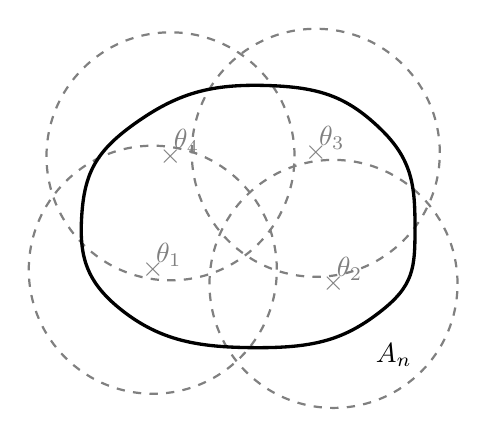
\begin{tikzpicture}[scale=0.9]
  \foreach \c/\r/\idx in {{(-1.2,-0.4)}/1.75/1, {(1.35,-0.6)}/1.75/2, {(1.1,1.25)}/1.75/3, {(-0.95,1.2)}/1.75/4} {
    \draw[gray, dashed, thick] \c circle (\r);
    \node[gray] at \c {$\times$};
    \node[gray, above right, inner sep=1pt] at \c {$\theta_{\idx}$};
  }
  \draw[very thick] plot[smooth cycle, tension=0.8] coordinates
    {(-2.2,0.4) (-1.4,1.7) (0.4,2.2) (2.0,1.6) (2.5,0.2) (2.0,-1.0) (0.3,-1.5) (-1.6,-1.0)};
  \node at (2.2,-1.6) {$A_n$};
\end{tikzpicture}
\end{center}
\end{intuition}

\begin{proof}[Proof of Theorem \ref{thm:tests}]
We do not fix the threshold $\Delta_n$ of the tests and the radius $\delta$ of the local balls now: as in an $\varepsilon$--$\delta$ proof, we write down the conditions they must satisfy along the way, as constraints $(\mathrm{C}_1), (\mathrm{C}_2), \dots$, and we solve this system at the end (Step 3). They may depend on $\varepsilon$ and $n$, but not on $\theta_1$ or $\theta$, so that all bounds are uniform.

\textbf{Step 1: Construction and expectation bound on local tests.}
\begin{leftbar}
Let $\theta_1 \in \gunderbrace{A_n := \Theta_n \cap \{\|f_\theta - f_{\theta_0}\| > \varepsilon\}}{\annot{will be used for Schwartz thm}}$,
\[ \phi_{n,\theta_1} := \ind\Big\{\sum_{i=1}^n \big(\ind_{R(\theta_1)}(X_i) - P_{\theta_0}(R(\theta_1))\big) > \Delta_n\Big\} \]
with $R(\theta_1) := \{x : f_{\theta_1}(x) > f_{\theta_0}(x)\}$ \annot{($A(\theta_1)$ in Rousseau's notes)}.

\textbf{Gap inequality.} Writing $R := R(\theta_1)$, we have
\[ P_{\theta_1}(R) - P_{\theta_0}(R) = \frac{1}{2}\|f_{\theta_1} - f_{\theta_0}\|_1 > \frac{\varepsilon}{2}. \qquad \text{(G)} \]
\begin{leftbar}
$\int (f_{\theta_1} - f_{\theta_0})\, d\mu = 1 - 1 = 0$, so $P_{\theta_1}(R) - P_{\theta_0}(R) = \int_R (f_{\theta_1} - f_{\theta_0})\, d\mu = \int_{R^c} (f_{\theta_0} - f_{\theta_1})\, d\mu$.

$f_{\theta_1} - f_{\theta_0} > 0$ on $R$ and $\le 0$ on $R^c$, so
\[ \|f_{\theta_1} - f_{\theta_0}\|_1 = \int_R (f_{\theta_1} - f_{\theta_0})\, d\mu + \int_{R^c} (f_{\theta_0} - f_{\theta_1})\, d\mu = 2\big(P_{\theta_1}(R) - P_{\theta_0}(R)\big), \]
which gives the equality; the inequality holds since $\theta_1 \in A_n$.
\end{leftbar}

\begin{intuition}[Intuition behind $\phi_{n,\theta_1}$]
If $\theta_1 \neq \theta_0$, by the way $R(\theta_1)$ is defined, the proba under $P_{\theta_1}$ for falling in $R(\theta_1)$ is much larger than the proba under $P_{\theta_0}$ to fall in $R(\theta_1)$. So
\[ \frac{1}{n}\sum_{i=1}^n \ind_{R(\theta_1)}(X_i) - P_{\theta_0}(R(\theta_1)) \xrightarrow[\text{LLN}]{}
\begin{cases}
> \frac{\varepsilon}{2} & \text{under } P_{\theta_1} \text{ (by (G))} \\
0 & \text{under } P_{\theta_0}
\end{cases} \]
i.e.\quad
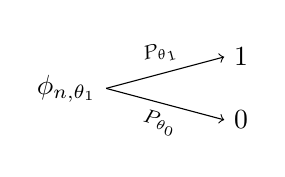
\begin{tikzpicture}[baseline=(phi.base)]
  \node (phi) {$\phi_{n,\theta_1}$};
  \draw[->] (phi.east) -- node[above, sloped] {$\scriptstyle P_{\theta_1}$} ++(1.5,0.4) node[right] {$1$};
  \draw[->] (phi.east) -- node[below, sloped] {$\scriptstyle P_{\theta_0}$} ++(1.5,-0.4) node[right] {$0$};
\end{tikzpicture}
\end{intuition}

\textbf{Step 1.1: Control of type I error} (i.e. $\mathbb{E}_{\theta_0}^{n}[\phi_{n,\theta_1}]$)
\begin{leftbar}
\[ \mathbb{E}_{\theta_0}^{n}[\phi_{n,\theta_1}] = P_{\theta_0}^{n}\Big(\sum \big(\ind_{R(\theta_1)}(X_i) - P_{\theta_0}(R(\theta_1))\big) > \Delta_n\Big) \]
\textbf{Hoeffding inequality:} if $Y_1, \dots, Y_n$ are $\perp\!\!\!\perp$ r.v. in
\begin{leftbar}
$[a_i, b_i]$ a.s. $\forall i \le n$ then $\forall t > 0$
\[ P\Big(\sum (Y_i - \mathbb{E}[Y_i]) \ge t\Big) \le \exp\Big(-\frac{2t^2}{\sum (b_i - a_i)^2}\Big) \]
\end{leftbar}
We use Hoeffding with
\[ Y_i = \ind_{R(\theta_1)}(X_i) - P_{\theta_0}(R(\theta_1)) \in \big[-P_{\theta_0}(R(\theta_1));\ 1 - P_{\theta_0}(R(\theta_1))\big] \]
and $t = \Delta_n$, which requires
\constraint{1}{\Delta_n > 0}
\ Then:
\[ \mathbb{E}_{\theta_0}^{n}[\phi_{n,\theta_1}] \le \exp\big(-2\Delta_n^2/n\big) \]
\end{leftbar}

\textbf{Step 1.2: Control of type II error} (i.e. $\sup_\theta \mathbb{E}_\theta^{n}[1 - \phi_{n,\theta_1}]$)
\begin{leftbar}
Let $\theta$ be s.t. $\|f_\theta - f_{\theta_1}\|_1 \le \delta$ (we will set $\delta$ later, so that it satisfies the constraints).
\begin{align*}
\mathbb{E}_\theta^{n}[1 - \phi_{n,\theta_1}] &= P_\theta^{n}\Big(\sum_{i=1}^{n} \ind_{R(\theta_1)}(X_i) - n P_{\theta_0}(R(\theta_1)) \le \Delta_n\Big) \\
&\qquad \annot{$\downarrow + n P_{\theta_0}(R(\theta_1)) - n P_\theta(R(\theta_1))$} \\
&= P_\theta^{n}\Big(\sum_{i=1}^{n} \ind_{R(\theta_1)}(X_i) - n P_\theta(R(\theta_1)) \\
&\qquad\qquad \le \Delta_n + n\big(P_{\theta_0}(R(\theta_1)) - P_\theta(R(\theta_1))\big)\Big)
\end{align*}
\textbf{(Reversed) Hoeffding inequality} (Proof: take $Y_i \leftarrow -Y_i$ in Hoeffding)
\begin{leftbar}
$[a_i, b_i]$ a.s. $\forall i \le n$ then $\forall t > 0$
\[ P\Big(\sum (Y_i - \mathbb{E}[Y_i]) \le -t\Big) \le \exp\Big(-\frac{2t^2}{\sum (b_i - a_i)^2}\Big) \]
\end{leftbar}
We want to use Hoeffding inequality with
\[ Y_i = \ind_{R(\theta_1)}(X_i) - P_\theta(R(\theta_1)) \in \big[-P_\theta(R(\theta_1));\ 1 - P_\theta(R(\theta_1))\big] \]
and $-t = \Delta_n + n\big(P_{\theta_0}(R(\theta_1)) - P_\theta(R(\theta_1))\big)$, so we need to have $t > 0$, i.e.
\begin{gather*}
\Delta_n + n\big(P_{\theta_0}(R) - P_\theta(R)\big) < 0 \\
\text{i.e.} \quad \Delta_n < n\big(P_\theta(R) - P_{\theta_0}(R)\big)
\end{gather*}


\textbf{Lower bound (not depending on $\theta$) of $P_\theta(R) - P_{\theta_0}(R)$}
\begin{leftbar}
($R := R(\theta_1)$)
\begin{align*}
P_\theta(R) - P_{\theta_0}(R) &= P_{\theta_1}(R) - P_{\theta_0}(R) + P_\theta(R) - P_{\theta_1}(R) \\
&= \underbrace{\int_R (f_{\theta_1} - f_{\theta_0})\, d\mu}_{= \frac{1}{2}\|f_{\theta_0} - f_{\theta_1}\|_1 \text{ by (G)}} + \gunderbrace{\int_R (f_\theta - f_{\theta_1})\, d\mu}{|\cdot| \le \frac{1}{2}\|f_{\theta_1} - f_\theta\|_1 \le \frac{\delta}{2}\ \annot{(cond. on $\theta$)}} \\
&\overset{}{\ge} \frac{1}{2}\|f_{\theta_0} - f_{\theta_1}\|_1 - \frac{\delta}{2}  \\
&{> \frac{\varepsilon - \delta}{2} \qquad \text{(by (G))}}
\end{align*}
This bound depends neither on $\theta$ nor on $\theta_1$.
\end{leftbar}
So $t > 0$ holds as soon as
\constraint{2}{\Delta_n < n\,\frac{\varepsilon - \delta}{2}}
and then, since $t > n\frac{\varepsilon - \delta}{2} - \Delta_n > 0$,
\[ \sup_{\theta \,:\, \|f_\theta - f_{\theta_1}\|_1 \le \delta} \mathbb{E}_\theta^{n}[1 - \phi_{n,\theta_1}] \le \exp\Big(-\frac{2}{n}\Big(n\,\frac{\varepsilon - \delta}{2} - \Delta_n\Big)^2\Big). \]
\end{leftbar}

\end{leftbar}

\medskip
\textbf{Step 2: Global control of type I and II errors}
\begin{leftbar}
By hypothesis, $\mathcal{P}_{\Theta_n}$ is covered by $N_n \le e^{n\varepsilon^2/16}$ balls of radius $\frac{\varepsilon}{4}$. In each ball meeting $\{f_\theta, \theta \in A_n\}$ we pick a new centre $f_{\theta_j}$ with $\theta_j \in A_n$ (needed in Step 1.2); the ball is then contained in $\{\theta : \|f_\theta - f_{\theta_j}\|_1 \le \frac{\varepsilon}{2}\}$. To apply Step 1.2 on these sets we need
\constraint{3}{\delta \ge \frac{\varepsilon}{2}}

Let $\phi_n := \max_{j \le N_n} \phi_{n,\theta_j}$.

\textbf{Step 2.1: Type I control:}
\begin{leftbar}
then
\[ \mathbb{E}_{\theta_0}^{(n)}[\phi_n] \le \sum_{j=1}^{N_n} \mathbb{E}_{\theta_0}^{(n)}[\phi_{n,\theta_j}] \le N_n\, e^{-2\Delta_n^2/n} \le \exp\Big(\frac{n\varepsilon^2}{16} - \frac{2\Delta_n^2}{n}\Big). \]
For Borel--Cantelli this must be summable, so the exponent must be negative (of order $-n$):
\constraint{4}{\Delta_n > n\,\frac{\varepsilon}{4\sqrt{2}}}
Then, since $\phi_n \in \{0, 1\}$, $\sum_n P_{\theta_0}(\phi_n = 1) < \infty$, and by Borel--Cantelli $\phi_n \xrightarrow[n\to\infty]{P_{\theta_0} \text{ a.s.}} 0$.
\end{leftbar}
\textbf{Step 2.2: Type II control:}
\begin{leftbar}
\begin{align*}
\sup_{\theta \in A_n} \mathbb{E}_\theta[1 - \phi_n] &= \sup_j \sup_{\theta : \|f_\theta - f_{\theta_j}\|_1 \le \delta} \mathbb{E}_\theta[1 - \phi_n] \\
&\le \sup_j \ {\sup_{\theta : \|f_\theta - f_{\theta_j}\|_1 \le \delta} \mathbb{E}_\theta[1 - \phi_{n,\theta_j}]} \\
&{\le \exp\Big(-\frac{2}{n}\Big(n\,\frac{\varepsilon - \delta}{2} - \Delta_n\Big)^2\Big)}
\end{align*}
\end{leftbar}
\end{leftbar}

\medskip
\textbf{Step 3: Solving the constraints}
\begin{leftbar}
\[ (\mathrm{C}_1)\ \Delta_n > 0, \qquad (\mathrm{C}_2)\ \Delta_n < n\,\frac{\varepsilon - \delta}{2}, \qquad (\mathrm{C}_3)\ \delta \ge \frac{\varepsilon}{2}, \qquad (\mathrm{C}_4)\ \Delta_n > n\,\frac{\varepsilon}{4\sqrt{2}}. \]
A small $\delta$ leaves more room in $(\mathrm{C}_2)$, so we take the smallest value allowed by $(\mathrm{C}_3)$: $\boxed{\delta = \frac{\varepsilon}{2}}$. The constraints on $\Delta_n$ become
\[ n\,\frac{\varepsilon}{4\sqrt{2}} < \Delta_n < n\,\frac{\varepsilon}{4}, \]
a non-empty interval since $\sqrt{2} > 1$. We take $\boxed{\Delta_n = \frac{n\varepsilon}{5}}$. Then:
\begin{itemize}
    \item type I: $\mathbb{E}_{\theta_0}^{(n)}[\phi_n] \le \exp\big(\frac{n\varepsilon^2}{16} - \frac{2n\varepsilon^2}{25}\big) = e^{-\frac{7}{400} n\varepsilon^2}$, so by Borel--Cantelli $\phi_n \to 0$ $P_{\theta_0}$ a.s.;
    \item type II: $\displaystyle\sup_{\theta \in A_n} \mathbb{E}_\theta(1 - \phi_n) \le \exp\Big(-\frac{2}{n}\Big(\frac{n\varepsilon}{4} - \frac{n\varepsilon}{5}\Big)^2\Big) = e^{-nC(\varepsilon)}$ with $C(\varepsilon) = \frac{\varepsilon^2}{200}$.
\end{itemize}
\end{leftbar}
\end{proof}

\noindent\textbf{Remark.} The $16$ of the entropy condition is what makes the system solvable: with $\frac{n\varepsilon^2}{8}$ instead, $(\mathrm{C}_4)$ would read $\Delta_n > \frac{n\varepsilon}{4}$, incompatible with $(\mathrm{C}_2)$.

\subsubsection{Hellinger Tests}

\begin{theorem}[Existence of Hellinger Tests]
\tocomplete
\end{theorem}

\begin{corollary}[Tests for the Hellinger Distance]
\tocomplete
\end{corollary}
\begin{proof}
\tocomplete
\end{proof}

\subsection{Parametric Models}
Let $X_1, \dots, X_n \overset{\text{iid}}{\sim} P_\theta$, $\theta \in \Theta \subset \mathbb{R}^p$.

Let $\pi$ be a prior on $\Theta$ with density w.r.t. the Lebesgue measure on $\mathbb{R}^p$ such that $\pi$ is strictly positive and continuous on $\Theta$. Assume that there exists a measure $\mu$ such that
\[ \forall \theta \in \Theta, \quad \frac{dP_\theta}{d\mu} = f_\theta. \]

\begin{theorem}[Consistency in Parametric Models] \label{thm:param}
Let $d(f_1, f_2) := \|f_1 - f_2\|_1$ or $d_H(f_1, f_2)$. If:
\begin{enumerate}
    \item $\exists\, \gamma_1 > 0,\ \delta > 0$ s.t. $\forall \theta \in \Theta$:
    \[ \|\theta - \theta_0\| < \delta \implies \KL(f_{\theta_0}, f_\theta) \le \|\theta - \theta_0\|^{\gamma_1} \]
    \item $\exists\, \gamma_2 > 0$ s.t. $d(f_{\theta_1}, f_{\theta_2}) \le \|\theta_1 - \theta_2\|^{\gamma_2}$
    \item $\exists\, \alpha > 0$ s.t. $\pi(\|\theta\| > x) \underset{x \to \infty}{\le} x^{-\alpha}$
\end{enumerate}
Then the posterior distribution is consistent at $\theta_0$ w.r.t. the metric $d$.
\end{theorem}
\begin{proof}
The proof consists in proving the three conditions of the posterior consistency lemma (Lemma \ref{lem:consistency}).

\textbf{K-L condition}
\begin{leftbar}
We want to show:
\[ \forall \varepsilon > 0, \quad \pi\big(\{\theta;\ \KL(f_{\theta_0}, f_\theta) < \varepsilon\}\big) > 0. \]
Let $\varepsilon > 0$. We will use condition 1:
\[ \|\theta - \theta_0\| < \delta \implies \KL(f_{\theta_0}, f_\theta) \le \|\theta - \theta_0\|^{\gamma_1} \]
And we have:
\[ \|\theta - \theta_0\|^{\gamma_1} < \varepsilon \iff \|\theta - \theta_0\| < \varepsilon^{1/\gamma_1} \]
So for all $\theta$ s.t. $\|\theta - \theta_0\| < \min(\delta, \varepsilon^{1/\gamma_1})$, we get
\[ \KL(f_{\theta_0}, f_\theta) \le \|\theta - \theta_0\|^{\gamma_1} < \varepsilon, \]
i.e.
\[ B\big(\theta_0, \min(\delta, \varepsilon^{1/\gamma_1})\big) \subset \{\theta : \KL(f_{\theta_0}, f_\theta) < \varepsilon\}. \]
And since $\mathrm{Vol}\big(B(\theta_0, \min(\delta, \varepsilon^{1/\gamma_1}))\big) > 0$, we have $\mathrm{Vol}\big(\{\theta;\ \KL(f_{\theta_0}, f_\theta) < \varepsilon\}\big) > 0$.

And since $\pi(x) > 0$ $\forall x \in \Theta$ and $\pi$ is continuous,
\[ \pi\big(\{\theta : \KL(f_{\theta_0}, f_\theta) < \varepsilon\}\big) > 0. \]
\end{leftbar}

\textbf{Covering condition}
\begin{leftbar}
Let $\Theta_n := \{\|\theta\| \le R_n\}$ with $R_n$ to be determined later. We want to prove that
\[ \log N\Big(\frac{\varepsilon}{4}, \mathcal{P}_{\Theta_n}, \|\cdot\|_1\Big) \le \frac{n\varepsilon^2}{16}. \]
\textbf{Let's prove that} $\forall u > 0$, $N(u, \mathcal{P}_{\Theta_n}, d) \le N(u^{1/\gamma_2}, \Theta_n, \|\cdot\|)$.
\begin{leftbar}
Let $u > 0$ and $N := N(u^{1/\gamma_2}, \Theta_n, \|\cdot\|)$, with $\theta_1, \dots, \theta_N$ the centers of the corresponding balls.

Let $\theta \in \Theta_n$: $\exists\, j \in \{1, \dots, N\}$ s.t. $\|\theta - \theta_j\| < u^{1/\gamma_2}$.

Recall assumption 2:
\[ \exists\, \gamma_2 > 0 \text{ s.t. } d(f_\theta, f_{\theta_j}) \le \|\theta - \theta_j\|^{\gamma_2}, \quad \text{i.e. } d(f_\theta, f_{\theta_j})^{1/\gamma_2} \le \|\theta - \theta_j\|. \]
So
\[ d(f_\theta, f_{\theta_j})^{1/\gamma_2} \le \|\theta - \theta_j\| \le u^{1/\gamma_2}, \quad \text{so} \quad d(f_\theta, f_{\theta_j}) \le u. \]
So by taking $N$ balls of radius $u$, we can cover $\mathcal{P}_{\Theta_n}$ w.r.t. the metric $d$. So by minimality of $N(u, \mathcal{P}_{\Theta_n}, d)$:
\[ N(u, \mathcal{P}_{\Theta_n}, d) \le N = N(u^{1/\gamma_2}, \Theta_n, \|\cdot\|). \]
\end{leftbar}
So if we find a way to control the covering number in the (Euclidean) space of parameters, we will control the covering number in the space of distributions.

\begin{proposition}[Covering Number of a Ball (not demonstrated)]
$\exists\, C > 0$ s.t. $\forall u > 0$, $\forall r > 0$:
\[ N\big(u, B(0, r), \|\cdot\|\big) \le \Big(\frac{rC}{u}\Big)^p \quad \text{in } \mathbb{R}^p. \]
\end{proposition}

So
\begin{align*}
\log N\Big(\frac{\varepsilon}{4}, \mathcal{P}_{\Theta_n}, \|\cdot\|_1\Big) &\le \log N\Big(\Big(\frac{\varepsilon}{4}\Big)^{1/\gamma_2}, \gunderbrace{\Theta_n}{\annot{$B(0, R_n)$}}, \|\cdot\|\Big) \\
&\overset{\annot{Prop}}{\le} \log\Bigg(\bigg(\frac{R_n C}{(\varepsilon/4)^{1/\gamma_2}}\bigg)^p\Bigg) = p \log R_n + \frac{p}{\gamma_2} \log\Big(\frac{4}{\varepsilon}\Big) + p \log C.
\end{align*}
So we want to have (asymptotically w.r.t. $n$):
\[ p \log R_n + \frac{p}{\gamma_2} \log\Big(\frac{4}{\varepsilon}\Big) + p \log C \le \frac{n\varepsilon^2}{16}. \]
Since $\frac{p}{\gamma_2} \log\big(\frac{4}{\varepsilon}\big) + p \log C$ does not depend on $n$, there exists $n_0$ such that it is $\le \frac{n\varepsilon^2}{32}$ for all $n \ge n_0$. So it suffices to have
\[ p \log R_n \le \frac{n\varepsilon^2}{32}, \]
which is equivalent to
\[ R_n \le \exp\Big(\frac{n\varepsilon^2}{32p}\Big). \]
We take
\[ R_n := \exp\Big(\frac{n\varepsilon^2}{32p}\Big) \xrightarrow[n\to\infty]{} +\infty \]
(we need $R_n \to \infty$ for the third condition). With this $R_n$ we obtain the covering condition: $\forall n \ge n_0$,
\[ \log N\Big(\frac{\varepsilon}{4}, \mathcal{P}_{\Theta_n}, \|\cdot\|_1\Big) \le \frac{n\varepsilon^2}{16}. \]
\end{leftbar}

\textbf{Control on $\pi(\Theta_n^c)$ condition}
\begin{leftbar}
Recall assumption 3:
\[ \exists\, \alpha > 0 \text{ s.t. } \pi(\|\theta\| > x) \underset{x \to \infty}{\le} x^{-\alpha}. \]
Since $R_n \to \infty$, we can use it with $x \leftarrow R_n = \exp\big(\frac{n\varepsilon^2}{32p}\big)$: for $n$ large enough,
\[ \pi\big(\gunderbrace{\Theta_n^c}{\annot{$\{\theta : \|\theta\| > R_n\}$}}\big) \le R_n^{-\alpha} = \exp\Big(-\frac{\alpha n\varepsilon^2}{32p}\Big). \]
Which gives the third condition and finally the posterior consistency lemma, which yields the result.
\end{leftbar}
\end{proof}

\begin{example}[Normal Location Model]
\tocomplete
\end{example}

\begin{example}[Uniform Model $\mathcal{U}({[0, \theta]})$]
\tocomplete
\end{example}

\section{Posterior Convergence Rate}

\subsection{Definitions and Theorem}

\begin{definition}[Posterior Contraction Rate]
\tocomplete
\end{definition}

\begin{intuition}
\tocomplete
\end{intuition}

\begin{theorem}[Posterior Contraction Rate] \label{thm:rate}
\tocomplete
\end{theorem}

\noindent\textbf{Remark (i.i.d.\ observations):} \tocomplete

\begin{lemma}[Lower Bound on $D_n$]
\tocomplete
\end{lemma}
\begin{proof}
\tocomplete
\end{proof}

\begin{proof}[Proof of Theorem \ref{thm:rate}]
\tocomplete
\end{proof}

\begin{proposition}[Key Inequality]
\tocomplete
\end{proposition}

\begin{corollary}[I.I.D.\ Case with the Hellinger or $L^1$ Distance]
\tocomplete
\end{corollary}
\begin{proof}
\tocomplete
\end{proof}

\subsection{Consequence on the Convergence of the Posterior Mean}
\tocomplete

\noindent\textbf{Remark (unbounded parameter space):} \tocomplete

\begin{example}[Contraction Rate in the Normal Location Model]
\tocomplete
\end{example}

\noindent\textbf{Exercise (contraction rate in linear regression):} \tocomplete

\noindent\textbf{Exercise (nonparametric regression):} \tocomplete

\end{document}